\chapter[Introduction]{Introduction}
\label{cp:introduction}

{
\parindent0pt

\textit{Authors: Edun Joshua, Mbuotidem Awak, Makinde Kayode}

% \textit{Current Version: 2.2.4}

\textit{License: \LaTeX~Project Public License v1.3c}

\textit{Official Repository: \href{https://github.com/joseareia/ipleiria-thesis}{GitHub Repository}}

\vspace{.935em}

\acrfull{phl} refers to the measurable reduction in the quantity or quality of food after harvest, making it unfit for consumption
 \citep{FAO_PostHarvest}. Globally, roughly one-third of food produced is lost or wasted. In Nigeria, the scope is especially alarming: studies estimate that the country loses on the order of 40–50\% of its total food production each year.



\begin{block}[note]
    \textit{“Each year, Nigeria wastes 40\% of its total food production”, equivalent to significant greenhouse gas emissions
    \citep{worldbank2020}.}
    \end{block}
    


 \section{Analysis of Post-Harvest Losses in Nigeria}   

According to \citet{NAN2024}, FAO experts similarly report losses around 50\% for certain crops. 
USAID reports that post-harvest losses for fresh produce in Nigeria can reach almost 50\% \citet{Udi2024}, and for tubers, fruits, and vegetables, losses can range between 50\% and 60\% \citep{OkojieJaiyesimi2024}.
These statistics reveal a gap between Nigeria’s agricultural output and what actually reaches consumers. \autoref{fig:figure-01} illustrates the estimated post-harvest losses for key crops in Nigeria, according to the APHLIS database \citep{APHLIS}.


\begin{figure}[H]
    \centering
    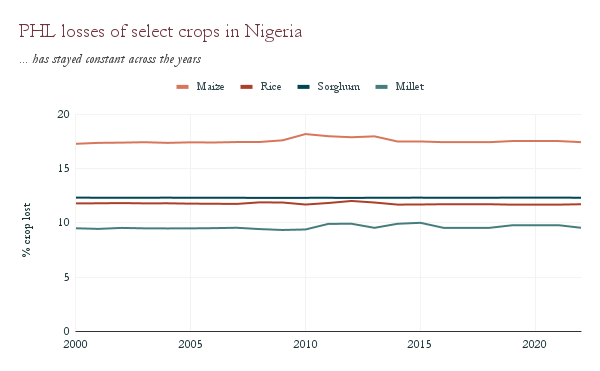
\includegraphics[scale=0.8]{Figures/phl_crops_v2.png}
    \caption{\acrshort{phl} in Nigeria for key crops. Source: APHLIS database, 2019}
    \label{fig:figure-01}
\end{figure}

\autoref{fig:figure-02} shows post-harvest losses across different value chain steps from 2018 to 2022. The total estimated loss peaked in 2019 at over 2.2 million tonnes, followed by slight declines in subsequent years. The highest losses consistently occurred during the harvesting/field drying and household-level storage phases, which together accounted for over half of total losses in all years.
Losses during further drying and threshing and shelling remained moderate but stable across the years. Transport from the field showed smaller but steady losses, while losses during transport to market and market storage were recorded as zero for all years, possibly due to either minimal losses or lack of data collection at those points. These trends suggest that targeted interventions in drying and storage practices could significantly reduce total post-harvest loss.

\begin{figure}[H]
    \centering
    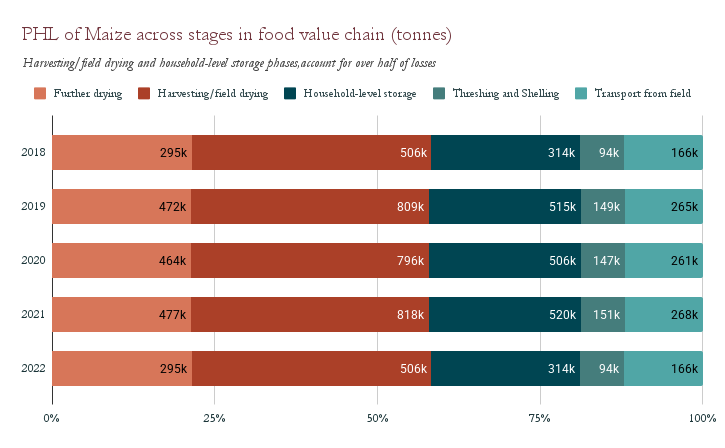
\includegraphics[scale=0.5]{Figures/phl_across_value_chain.png}
    \caption{\acrshort{phl} loss in the various steps in the maize value chain. Source: APHLIS database, 2019}
    \label{fig:figure-02}
\end{figure}

PHL is not just loss of food; it translates to loss in precious nutritional value. Maize for example is a staple food in Nigeria and PHL losses mean less nutrients for people. The data shows that, the amount of nutrients lost from PHL, equivalent to the average person's dietary requirements has been on the rise since the 2000s as \autoref{fig:figure-03} shows.

\begin{figure}[H]
    \centering
    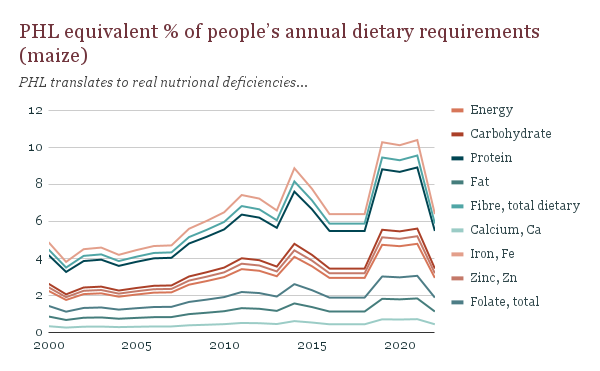
\includegraphics[scale=0.7]{Figures/phl_nutritional_maize.png}
    \caption{\acrshort{phl} expressed in the percentage of the average person's annual dietary requirements}
    \label{fig:figure-03}
\end{figure}


Analysis of \acrshort{phl} loss in maize in 2022 is summarised in \autoref{tab:table-01}. For instance, the post-harvest loss of approximately 4.8 trillion kcal of energy and 878 million kg of carbohydrate alone could have met the annual energy and carbohydrate requirements of over 5.7 million and 6.7 million people, respectively, across the total Nigerian population. These losses represent 2.9\% and 3.5\% of the total population's annual requirements for energy and carbohydrate. This is an obvious symptom of inefficiency in the food system that prevents available nutrients from reaching consumers.

The nutritional impact is particularly pronounced for vulnerable demographic groups, such as males aged 9-13 years. Within this focal group, the lost maize could have fulfilled the annual protein requirements for nearly 12.7 million individuals, a figure exceeding the total population of this demographic in 2022. This translates to a staggering 98.4\% of the focal group's annual protein needs that were not met due to post-harvest losses. 
% Similarly, the losses of essential micronutrients like Iron and Zinc also demonstrate critical impacts on this age group, representing 102.5\% and 46.3\% of their annual requirements, respectively. 
% While the lost quantities of some nutrients like Vitamin A and Vitamin C were negligible in maize for this period, the substantial losses of protein, iron, and zinc underscore how post-harvest issues directly exacerbate micronutrient deficiencies and food insecurity among vulnerable populations in Nigeria. 
% Addressing these losses is therefore critical not only for improving food availability but also for improving the nutritional status of the population, particularly among children and adolescents.
\begin{table}[h!]
    \centering
    \caption{Nutritional Impact of Maize Post-Harvest Losses in Nigeria, 2022}
    \label{tab:table-01}
    % Use tabularx with \textwidth for the total width
    % Define columns: l, r, and L for wrapping columns
    
    \begin{tabularx}{\textwidth}{|l|r|L|L|L|L|}
        \hline
        \multirow{2}{*}{Nutrient} & \multirow{2}{*}{Quantity lost postharvest} & \multicolumn{2}{c|}{Total population, Nigeria} & \multicolumn{2}{c|}{Male, 9-13 years, Nigeria} \\
        \cline{3-6}
         &  & Number of people's annual nutritional requirements lost & \% of population nutritional requirements lost & Number of people in focal group's annual nutrient requirements lost & \% of focal group population's annual nutritional requirements lost \\
        \hline
        Energy & 4,797,678,189 kcal & 5,771,644 & 2.9 & 5,752,439 & 44.7 \\
        Carbohydrate & 878,428,757 kg & 6,763,242 & 3.5 & 6,740,738 & 52.4 \\
        Protein & 126,471,746 kg & 10,744,369 & 5.5 & 12,664,398 & 98.4 \\
        Fat & 56,362,409 kg & 2,214,600 & 1.1 & 2,211,670 & 17.2 \\
        Fibre, total dietary & 133,345,210 kg & 11,522,627 & 5.9 & 11,420,111 & 88.8 \\
        Calcium, Ca & 261,192 kg & 864,988 & 0.442 & 650,540 & 5.1 \\
        Iron, Fe & 42,615 kg & 12,528,603 & 6.4 & 13,192,626 & 102.5 \\
        Zinc, Zn & 21,308 kg & 6,266,152 & 3.2 & 5,956,874 & 46.3 \\
        Folate, total & 357.4 kg & 3,686,759 & 1.9 & 3,916,933 & 30.4 \\
        Vitamin A (RAE) & 0 kg & 0 & 0 & 0 & 0 \\
        Vitamin C & 0 kg & 0 & 0 & 0 & 0 \\
        \hline
    \end{tabularx}
\end{table}

\acrshort{phl} also reflects as financial loss. Between 2013 and 2020, the financial impact of rice PHL grew from \$536,467,825 in 2013 to \$970,343,075 in 2020.

While the losses remained below 1\% of the national agricultural GDP, the rising absolute value calls for attention to mitigation strategies to alleviate the effects on farmer's income, availability of rice to consumers and overall economic stability.


\begin{figure}[H]
    \centering
    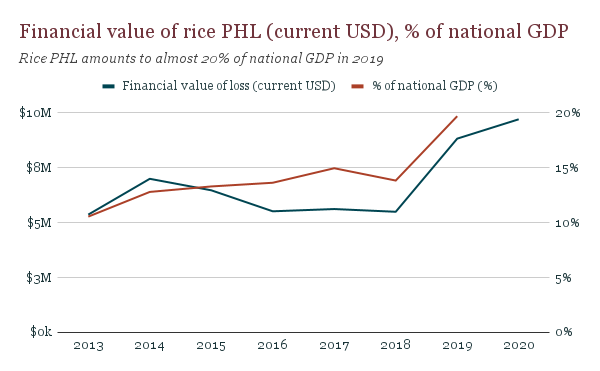
\includegraphics[scale=0.7]{Figures/phl_rice_financial_value.png}
    \caption{Financial value of rice PHL loss in Nigeria from 2013 to 2020. Source: APHLIS database, 2019}
    \label{fig:figure-04}
\end{figure}



\section{Impact on Youth and National Economy}

\acrshort{phl} have far-reaching consequences for Nigeria’s economy and youth engagement in agriculture. Economically, \acrshort{phl}  represents wasted farmer income and lost food value, with maize losses alone accounting for approximately 0.9\% of agricultural GDP. Furthermore, the inefficiency in food production results in under-utilized land—31\% of Nigeria’s cropland—and contributes to 5\% of the country’s greenhouse gas emissions. These losses inflate food prices, exacerbate food insecurity, and weaken national economic stability.

Beyond economic concerns, PHL directly affects Nigeria’s youth, the largest segment of the population. The agricultural sector, despite its substantial contribution to the GDP (around 24\%), is dealing with a dwindling workforce due to an aging farming population and the discouraging effects of post-harvest losses. Young people, who could drive innovation and modernization in agriculture, often view the sector as unappealing due to the visible waste and financial risks. Watching hard-earned produce deteriorate before reaching consumers discourages entrepreneurial efforts and limits agriculture’s potential as a viable career path.

Reducing post-harvest losses is therefore crucial to stabilizing the economy and making agriculture more attractive to younger generations. It would increase food availability without requiring expansion of farmland, improve farmers’ livelihoods, and foster a more resilient food system. Addressing PHL could encourage youth participation in agriculture, helping Nigeria move toward food self-sufficiency and boosting export potential. In essence, tackling post-harvest waste is not just about protecting farmers—it’s about securing Nigeria’s future.nd \(iv)\) designing it to be user-friendly, especially for newcomers.
}